\section{Introduction} 
 
Fluid-elastic galloping is one of the sub-areas of research in fluid structure interactions. This area has been of interest due to the vibrations crated by galloping on transmission lines and civil structures and leading them to failure. Therefore understanding this phenomenon in order to suppresses these vibrations was quite important. However, the search for alternate energy sources with minimal environmental impact has become an important area of research in the modern word. Therefore researchers are moving towards investigating the possibility of extracting useful energy from this vibrations rather than suppressing them. Thus, it is quite important to understand the governing parameters and analyse the influence of them on the energy transfer from the fluid to the structure, because this understanding will lead to develop better practical applications. Hence, in this paper we focus on understanding the energy transfer from the fluid to the body and isolate the governing parameters influencing it.

According to \citet{Paidoussis2010}, \citet{Glauert1919} provided a criterion for galloping by considering the auto-rotation of an aerofoil.  \citet{DenHartog1956} provided a theoretical explanation for galloping for iced electric transmission lines. A weakly non-linear theoretical aeroelastic model to predict the response of galloping was developed by \citet{Parkinson1964} based on the quasi-steady state hypothesis. Experimental lift and drag data on a fixed square prism at different angles of attack were used as an input for the theoretical model. It essentially used a curve fit of the transverse force to predict the galloping response. The study managed to achieve a good agreement with experimental data.

However, the QSS model equation when solved analytically using the sinusoidal solution, cannot predict the response for cases with low mass ratios. \citet{Joly2012} observed that finite element simulations show a sudden change in amplitude below a critical value of the mass ratio. The quasi-oscillator equation in \citet{Parkinson1964} was altered to account for the vortex shedding and solved numerically to predict the reduced displacement amplitude at low mass ratios to the point where galloping is no longer present. \citet{Barrero-Gil2010a} investigated the possibility of extracting power from vibrations caused by galloping using the quasi-steady state model. So far the studies on galloping using quasi-steady state assumption has been mainly focused on understanding the behaviour of the displacement amplitude. Although, it is quite important to analyse the behaviour of the velocity when studying the power transfer from the fluid to the body. This is because power could be simply defined as the product the force and velocity. This study also focuses on how well the QSS model perform at high damping at low Reynolds numbers. 


Here, the modified QSS model is integrated numerically for low Reynolds numbers. The power transfer from the fluid to the structure and the influence of mechanical parameters was investigated (i.e. mass, stiffness and damping). To this end, a series of previously mentioned mechanical parameters are tested at two different values of \reynoldsnumber: $\reynoldsnumber = 200$, a case that should remain laminar and closer to two-dimensional behaviour; $\reynoldsnumber = 22300$, a case where the flow is expected to be turbulent and three-dimensional. Both cases require the input of transverse force coefficients $C_y$ as a function of angle of attack $\theta$ for a fixed body. These data are provided from direct numerical simulations for the $\reynoldsnumber = 200$ case, while the data provided by \citet{Parkinson1964} are used for the $\reynoldsnumber = 22300$ case.

The structure of the paper is as follows. Section \ref{sec:theory} presents the governing equations and the oscillator model used to obtain data and introduces the method for the calculation of the power transferred from the fluid to the structure. Section \ref{sec:results} introduces the governing parameters namely, the combined mass-stiffness and the combined mass-damping obtained using linearised time scales of the oscillator model. The fixed body tests at a range of $\theta$ followed by the response characteristics predicted by the integration of the QSS model for both the high and low \reynoldsnumber\ cases. For the low \reynoldsnumber\ case, the results of the QSS model are compared to those of full direct numerical simulations of the fluid-structure interaction problem. Finally, section \ref{sec:conc} presents the conclusions that can be drawn from this work.
% % % % % % % % % % % % % % % % % % % % % % % % % % % % % % % % % % % % % % % % % % % % % % % % % % % % % % % % % % % % % % % % % % % % % % % % 
\section*{Nomenclature}
%\textbf{Nomenclature}

\begin{tabular}{ll}
$a_1,a_3,a_5,a_7$ & coefficients of the polynomial to determine $C_y$ \\ 
$A$ & displacement amplitude\\
$c$ & damping constant \\
$D$ & characteristic length (side length) of the cross section of the body \\
$f=\sqrt{k/m}/2\pi$ & natural frequency of the system \\
$F_y$ & instantaneous force normal to the flow \\ 
$F_0$& amplitude of the oscillatory force due to vortex shedding \\
$k$ & spring constant \\
$m$ & mass of the body \\
$m_a$ & added mass \\
$P_d$ & power dissipated due to mechanical damping  \\
$P_{in}=\rho U^3D/2$ & Energy flux of the approaching flow \\
$P_{mean}$ & mean power \\
$P_t$   & power transferred to the body by the fluid \\
$t$ & time \\
$U$ & freestream velocity \\
$U_i$ & Induced velocity \\
$y,\dot{y},\ddot{y}$ & transverse displacement, velocity and acceleration of the body \\
$\mathcal{A}=DL$ & frontal area of the body\\ 
$\lambda$ & Inverse time scale of a galloping dominated flow \\
$\lambda_{1,2}$ & Eigenvalues of linearized equation of motion \\
$\rho$ & fluid density  \\
$\omega_n= 2 \pi f$ & natural angular frequency of the system  \\
$\omega_s$ & vortex shedding angular frequency \\
$\cstar=cD/mU$ & non-dimensionalised damping factor \\
$C_y=F_y/0.5\rho U^2DL$ & normal (lift) force coefficient \\
$m^*=m/\rho D^2L$ & mass ratio \\
$Re$ & Reynolds number  \\
$U^*=U/fD$ & reduced velocity  \\
$Y=y/D$ & non-dimensional transverse displacement \\
$\dot{Y}=m^*\dot{y}/a_1U$ & non-dimensional transverse velocity \\
$\ddot{Y}=m^{*2}D/a_1^2U^2$ & non-dimensional transverse acceleration \\
$\Gamma_1 = 4\pi^2m^{*2}/U^{*2}a_1^2$ & First dimensionless group arising from linearised, non-dimensionalised equation of motion\\
$\Gamma_2 = c^*m^*/a_1$ & Second dimensionless group arising from linearised, non-dimensionalised equation of motion\\
$\zeta= c/2 m \omega_n$ & damping ratio \\
$\theta= \tan^{-1}{(\dot{y}/U)}$ & instantaneous angle of incidence (angle of attack)\\
$\massstiff =  4\pi^2m^{*2}/U^{*2}$ & Combined mass-stiffness parameter\\
$\massdamp = c^*m^*$ & Combined mass-damping parameter\\
\end{tabular}  


% % % % % % % % % % % % % % % % % % % % % % % % % % % % % % % % % % % % % % % % % % % % % % % % % % % % % % % % % % % % % % % % % % % % % % % % % % % %

\section{Problem formulation and methodology}
\label{sec:theory}

\subsection{The quasi-steady state (QSS) model}

The equation of motion of the body is given by 
\begin{equation}
\label{equationofmotion}
(m)\ddot{y}+c\dot{y}+ky=F_y,
\end{equation}
where the forcing term $F_y$ is given by
\begin{equation}
\label{lift equation}
F_y=\frac{1}{2}\rho U^2\mathcal{A}C_y.
\end{equation}


\begin{figure}[!h]
\setlength{\unitlength}{\textwidth}

  \begin{picture}(1,0.36)(0,0.74)
    
  \put(0.2,0.76){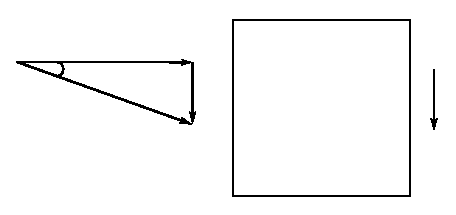
\includegraphics[width=0.5\unitlength]{./chapter-literature-revirw/fnp/setup-1.eps}}         
      
      
   
 	\put(0.315,1.04){$U$}
 	\put(0.3,0.95){$U_i$}
    \put(0.42,1.0){$\dot{y}$}
    \put(0.28,1.003){ $\theta$}
    \put(0.7,0.99){\small $(+)$}
      	

 	
 	 

     

  \end{picture}

 \caption{Induced angle of attack on a square prism due to the resultant of free-stream velocity of the fluid and transverse velocity of the body.}
    \label{fig:induced_lift_sketch}
\end{figure}

In the QSS model, it is assumed that the force on the body at a given instantaneous incident angle $\theta$ (defined in figure \ref{fig:setup_1}) is the same as the mean force on a static body at the same incident angle, or angle of attack. The instantaneous value of $C_y$ is therefore determined by an interpolating polynomial based on the lift data for flow over a stationary body at various $\theta$. Using the relationship between $\theta$ and the instantaneous transverse velocity of the body $\dot{y}$ shown in figure \ref{fig:setup_1}, $C_y$ can be written as a function of $\dot{y}$. The order of the interpolation polynomial used to define this function has varied from study to study. For  example a $7^{th}$ order polynomial was used in \cite{Parkinson1964} and $3^{rd}$ order polynomial was used in \cite{Barrero-Gil2009}. \cite{Ng2005} concluded that using a $7^{th}$ order polynomial is sufficient and a polynomial higher than that of $7^{th}$ order doesn't provides a significantly better result. Thus a $7 ^{th}$ order interpolating polynomial is used in this present study. As a result, $C_y(\theta)$ (noting that theta is proportional to $\dot{y}/U$) is defined as
\begin{equation}
\label{cy ploynomial}
C_y(\theta)=a_1\left(\frac{\dot{y}}{U}\right)+a_3\left(\frac{\dot{y}}{U}\right)^3+a_5\left(\frac{\dot{y}}{U}\right)^5+a_7\left(\frac{\dot{y}}{U}\right)^7.
\end{equation}

%\begin{equation}
%\label{modified_equation_of_motion}
%\ddot{y}+c^*\dot{y}+k^*y=\frac{1}{2}\rho U^2A
%\end{equation}

 It is expected that vortex shedding will be well correlated along the span and provide significant forcing at low \reynoldsnumber. \citet{Joly2012} introduced  an additional sinusoidal forcing function to the hydrodynamic forcing to model this. This enables the model to provide accurate predictions even at low mass ratios where galloping excitation is suppressed or not present. However, in this study we also focus on isolating the regions where the QSS model predicts well and therefore the additional sinusoidal forcing function is disregarded.  
 
 
 
\begin{equation}
\label{final_equation_motion}
m\ddot{y}{+}c\dot{y}{+}ky{=}\frac{1}{2}\rho U^2 \mathcal {A} \Bigg(a_1\left(\frac{\dot{y}}{U}\right){+}a_3\left(\frac{\dot{y}}{U}\right)^3{+}a_5\left(\frac{\dot{y}}{U}\right)^5{+}a_7\left(\frac{\dot{y}}{U}\right)^7.
\end{equation}

This equation can be solved using standard time integration methods. In this study the fourth-order Runge-Kutta scheme built in to the MATLAB routine `ode45' was generally used to obtain the solutions. 

\subsection{Calculation of average power}

 The dissipated power due to the mechanical damping represents the ideal potential amount of harvested power output. Therefore, the mean power output can be given by
\begin{equation}
\label{power}
P_{mean}=\frac{1}{T}\int_{0}^{T}(c\dot{y})\dot{y} dt,
\end{equation}
where $T$ is the period of integration and $c$ is the mechanical damping constant. 

It should be noted that this quantity is equal to the work done on the body by the fluid, defined as
\begin{equation}
\label{power_alt}
P_{mean}=\frac{1}{T}\int_{0}^{T}F_y\dot{y} dt,
\end{equation}
where $F_y$ is the transverse (lift) force.

 \hilight{have to repharase} These two definitions show two important interpretations of the power with respect to any energy production device. The first shows that power will be high for situations where the damping coefficient is high, and the transverse velocity is consistently high. The second shows that power will be high for situations where the transverse force and the body velocity are in phase.
 
 \begin{figure}

  \setlength{\unitlength}{\textwidth}
  \begin{picture}(1,0.25)(0,0.8)
  
    % % %90
      \put(0.025,0.81){\includegraphics[width=0.5\unitlength]{../FnP/gnuplot/lift_curve_200.eps}}
      \put(0.495,0.81){\includegraphics[width=0.5\unitlength]{../FnP/gnuplot/lift_curve_park.eps}}
 	\put(0.02,0.93){ \large $C_y$} 	
% 	\put(0.56,1.02){ $\theta$}
 	
        \put(0.25,0.8){ $\theta$} 	
        \put(0.75,0.8){ $\theta$}
        
        \put(0.117,1.01){(a)}
        \put(0.565,1.01){(b)}
      \end{picture}

  \caption{Lift coefficient, $C_y$, as a function of incidence angle $\theta$, for a static square cross section. (a) Data from simulations at $Re=200$  (b) data from \cite{Parkinson1964} at $Re=22300$. Points ($\bullet$) are measurements from the simulations. At $\reynoldsnumber=200$. Curves in both plots are 7th-order interpolating polynomials used to predict the fluid forcing for the QSS model. $C_y$ is the force coefficient of the force which occurs normal to the induced velocity.}
    \label{fig:lift_curves}
\end{figure}


 \begin{table}[ht]

\begin{center}
\setlength{\unitlength}{\textwidth}

\begin{tabular}{c c c c c} % centered columns (4 columns)
\hline\hline %inserts double horizontal lines
\\[0.2ex]
$\ratio$ & $a_1$ & $a_3$ & $a_5$ & $a_7$ \\ [0.8ex] % inserts table 
%heading
\hline 

\\[0.8ex]% inserts single horizontal line
$0$ &  -2.30617 & -269.075 & -59.2929 & 4.74389\\[0.8ex]
    & -5.08342 & -56.5390e & -160.505e & -105.773\\[0.8ex]
    &  4.40685 & 19.9213 & 22.8894 & 7.68556\\[1ex]


\\[0.8ex]% inserts single horizontal line
$0.25$ & -0.605146 & -19.4346 &-82.4463 & -94.4226\\[0.8ex]
      & 2.50538 & 9.91021  & 10.2712 & 3.94112 \\[1ex]

 \\[0.8ex]% inserting body of the table


 $0.5$ & 1.44734 & 4.83885  & -166.900e & -983.072 \\[0.8ex]% inserting body of the table
  & 1.51455e & 15.8476 & 52.5465 & 62.8067 \\ [1ex] % [1ex] adds vertical space
  
  \\[0.8ex]% inserting body of the table
  
   $0.75$ & 1.76938 & 35.2630 & -345.562 & -10072.7 \\[0.8ex]
          & 1.77553 & 43.0120 & 262.983 & 638.484 \\ [1ex]
          
          
  
  
\hline %inserts single line


\end{tabular}

\caption{Coefficient values used in the 7th order interpolation polynomial at $Re=200$. Data present for $\ratio=0-0.75$ at increments of $0.5$. Multiples polynomials were used to attain a better fit. The plot of the compound fit is presented in figure \ref{fig:lift_curves-hybrid}.} 
 
\label{table:cy-coefficients-hybrid} % is used to refer this table in the text
\end{center}
\end{table}


 
 \subsection{Parameters used} 
  
 For the low \reynoldsnumber\ tests, $\reynoldsnumber=200$ was maintained. Stationary $C_y$ data were obtained at different angles of attack ranging from $0^\circ$ to $16^\circ$. The average power was obtained by using equation \ref{power}, and the averaging was done over no less than 20 galloping periods. Predictions of power output at $\reynoldsnumber=22300$ were obtained using the coefficients for curve fitting $C_y$ (Table (\ref{table:cy-coefficients})) from \citet{Parkinson1964}, in order to provide a comparison between high and low Reynolds numbers. The mass ratio $m^*$ was kept at 1163 for $\reynoldsnumber=22300$ (Similar to \citet{Parkinson1964}) and $m^*=20$ for \reynoldsnumber=200. These parameters were used throughout this study unless otherwise specified. 
 
 The stationary data and the fluid-structure interaction (FSI) data were obtained using a high-order spectral element routine to simulate the two-dimensional laminar flow.  Simulations involving fluid structure interaction (FSI) were used to provide additional validation of the QSS model. The inlet was placed $20D$ while the outlet situated $60D$ away from the centroid of the body. The side boundaries were placed $20D$ away from the centroid of the body where $D$ was kept as unity throughout this study. The Navier--Stokes equations were solved in an accelerated frame of reference attached to the moving body along with the body equation of motion given in equation \ref{equationofmotion}. A three-step time splitting scheme together with high-order Lagrangian polynomials were used to obtain the solution. The details of the method can be found in \citet{Thompson2006,Thompson1996a}. This code has been very well validated in a variety of fluid-structure interaction problems \citep{Leontini2007a,Griffith2011,Leontini2011,Leontini2013}.
  
 The computational domain consists of 751 quadrilateral macro elements where the majority of the elements were concentrated near the square section. A freestream condition was given to the inlet, top and bottom boundaries and the normal velocity gradient was set to zero at the outlet. A convergence study was performed by changing the order of the polynomial ($p$-refinement) at $U^*=40$ and $\reynoldsnumber=200$. A $9^{th}$ order polynomial together with a time step of $\Delta tU/D=0.001$ was sufficient to ensure an accuracy of $2\%$ with regards to amplitude of oscillation.
 
 
 
 % % % % % % % % % % % % % Time scales % % % % % % % % % % % % % % % % % % % % % % % % % % % % % % %
 
 \section{Results}
  \label{sec:results}
  
     Figure \ref{fig:lift_curves} shows the plots of the interpolation polynomials as a function of $\theta$. For high \reynoldsnumber \ the polynomial incorporated by \cite{Parkinson1964} was used. For low \reynoldsnumber \ two polynomials were used to obtain a better fit to the data. One to fit data from $\theta=0^0 \rightarrow 7^0$ and the other $\theta > 7^0$ 
   there are several differences that can be observed when the low \reynoldsnumber\ data are compared with the $7^{th}$ order polynomial curve at $\reynoldsnumber=22300$ shown in figure \ref{cy ploynomial}(b). The peak value of $C_y$ is  significantly lower at $\reynoldsnumber=200$ ($C_y=0.12$ at $5^\circ$) in comparison with $\reynoldsnumber=22300$ ($C_y=0.57$ at $13^\circ$) . The inflection point present around $8^\circ$ for $\reynoldsnumber=22300$ is not observed at $\reynoldsnumber=200$. This agrees with the findings of \cite{Luo2003}.  It was concluded by \cite{Luo2003} that hysteresis in the system response occurs due to the inflection point in the $C_y$ curve. Therefore hysteresis is not expected at $\reynoldsnumber=200$.
  
   
  The range of incident flow angles where $C_y$ remains positive is narrow at $\reynoldsnumber=200$ ($0^\circ <\theta \leq$ $7^\circ$) compared to $\reynoldsnumber=22300$ ($0^\circ <\theta \leq 15^\circ$). This feature is what sustains galloping. Power is only transferred from the fluid to the supporting structure within this range of incident angles because fluid forces are acting in the direction of travel of the oscillating body, as demonstrated by equation \ref{power_alt}. Incident angles beyond this range actually suppress the galloping and power goes in the opposite direction, i.e; from body to fluid. Therefore due to the overall smaller $C_y$ and narrow range of angles where $C_y$ is positive for $\reynoldsnumber=200$ compared to $\reynoldsnumber=22300$, it is expected that the transferred power at $\reynoldsnumber=200$ is significantly lower than at $\reynoldsnumber=22300$.
  
 

 % % % % % % % % % % % % % % % % % % % % % % % % % % % % % % % % % %
  The natural time scales of the system can be found by solving for the eigenvalues of the linearised equation of motion, namely
 \begin{equation}
 \label{eqn:eom_linear}
 (m)\ddot{y}{+}c\dot{y}{+}ky{=}\frac{1}{2}\rho U^2 \mathcal{A} a_1\left(\frac{\dot{y}}{U}\right),
 \end{equation}
 which is simply the equation of motion presented in equation \ref{final_equation_motion} with the polynomial series for the lift force truncated at the linear term, and the forcing term representing vortex shedding removed.
 
 Combining the $\dot{y}$ terms and solving for eigenvalues gives
 \begin{equation}
   \label{eqn:eigs}
   \lambda_{1,2}= -\frac{1}{2}\frac{c-\frac{1}{2}\rho U\mathcal{A}a_1}{(m)}\pm\frac{1}{2}\sqrt{\left[\frac{c-\frac{1}{2}\rho U\mathcal{A}a_1}{(m)}\right]^2-4\frac{k}{(m+m_a)}}.
 \end{equation}
 
 If it is assumed that the spring is relatively weak, $k\rightarrow 0$, a single non-zero eigenvalue remains. This eigenvalue is
 \begin{equation}
   \label{eqn:eigs_nospring}
   \lambda=-\frac{c-\frac{1}{2}\rho U\mathcal{A}a_1}{(m)}.
 \end{equation}
 
 Further, if it is assumed that the mechanical damping is significantly weaker than the aerodynamic forces on the body, $c\rightarrow 0$ and
 \begin{equation}
   \label{eqn:eigs_nospring_nodamp}
   \lambda=\frac{\frac{1}{2}\rho U\mathcal{A}a_1}{(m)}.
 \end{equation}
 

 In this form, $\lambda$ represents the inverse time scale of the motion of the body due to the negative damping effect of the long-time aerodynamic forces. In fact, the terms can be regrouped and $\lambda$ written as
 \begin{equation}
   \label{eqn:timescale}
   \lambda = \frac{a_1}{m^*}\frac{U}{D}
 \end{equation}
 
 Written this way, the important parameters that dictate this inverse time scale are clear. The rate of change in the aerodynamic force with respect to angle of attack when the body is at the equilibrium position, $\partial C_y/\partial \alpha$, is represented by $a_1$. The mass ratio is represented by $m^*$. The inverse advective time scale of the incoming flow is represented by the ratio $U/D$. Increasing $a_1$ would mean the force on the body would increase more rapidly with small changes in the angle of attack, $\theta$, or transverse velocity. Equation \ref{eqn:timescale} shows that such a change will increase the inverse time scale, or analogously decrease the response time of the body. Increasing the mass of the body, thereby increasing $m^*$, has the opposite effect. The inverse time scale is decreased, or as might be expected, a heavier body will take longer to respond.
 
 This timescale can then be used to non-dimensionalize the equation of motion, and to find the relevant dimensionless groups of the problem. If the non-dimensional time, $\tau$, is defined such that $\tau=t(a_1/m^*)(U/D)$, the equation of motion presented in equation \ref{final_equation_motion} can be non-dimensionalized as
 \begin{equation}
   \label{eqn:eom_nondim}
   \ddot{Y} + \frac{m^{*2}}{a_1^2}\frac{kD^2}{mU^2}Y = \left(\frac{1}{2} - \frac{m^*}{a_1}\frac{cD}{mU}\right)\dot{Y} + H.O.T.,
 \end{equation}
 
 where $H.O.T.$ represents the higher order terms in $\dot{Y}$. The coefficients can be regrouped into combinations of non-dimensional groups, and rewritten as
 \begin{equation}
   \label{eqn:eom_nondim_regroup}
   \ddot{Y} + \frac{4\pi^{2}m^{*2}}{U^{*2}a_1^2}Y = \left(\frac{1}{2} - \frac{c^*m^*}{a_1}\right)\dot{Y} + H.O.T,
 \end{equation}
 
 where $c^*=cD/mU$ is a non-dimensional damping parameter.
 
 Equation \ref{eqn:eom_nondim_regroup} shows there are four non-dimensional parameters that play a role in setting the response of the system. These are the stiffness (represented by the reduced velocity $U^*$), the damping $c^*$, the mass ratio $m^*$, and the geometry, represented by the rate of change in the aerodynamic force with respect to angle of attack when the body is at the equilibrium position, $a_1$. The grouping of these parameters into two groups in equation \ref{eqn:eom_nondim_regroup} which arise by non-dimensionalising using the natural time scale of the galloping system, suggests there are two groups that dictate the response: $\Gamma_1 = 4\pi^2m^{*2}/U^{*2}a_1^2$ and $\Gamma_2 = c^*m^*/a_1$. For a given geometry and Reynolds number, $\Gamma_1$ can be thought of as a combined mass-stiffness, whereas $\Gamma_2$ can be thought of a a combined mass-damping parameter. As it is assumed that during galloping the stiffness plays only a minor role, $\Gamma_2$ seems a likely parameter to collapse the data presented in figure \ref{fig:uncollapsed_data}. In fact, in the classic paper on galloping from \citet{Parkinson1964}, galloping data from wind tunnel tests is presented in terms of a parameter that can be shown to be the same as $\Gamma_2$.
 
 All of the quantities that make up $\Gamma_1$ and $\Gamma_2$ can, in theory, be known before an experiment is conducted. However, the quantity $a_1$ is a relatively difficult one to determine, requiring static body experiments or simulations. Here, the geometry is unchanged and results are only being compared at the same \reynoldsnumber. Hence, suitable parameters can be formed by multiplying $\Gamma_1$ and $\Gamma_2$ by $a_1^2$ and $a_1$ respectively, to arrive at a mass-stiffness parameter $\massstiff =  4\pi^2m^{*2}/U^{*2}$, and a mass-damping parameter defined as $\massdamp = c^*m^*$.
 
 % % % % % % % % % % % % % % % % % % % % % % % % % % % % % % % % % % % % % % % % % % % % % % %
 
%   \input{../figure/collapsed_dta}
  
   Figure \ref{fig:collapsed_data} shows the comparison of mean power data presented using different independent variables. Sub-figure (a) and (c) shows the displacement and velocity amplitudes respectively and the (e) shows the mean power as a function of the classic VIV parameter, \ustar. (b), (d) and (f) shows the same data presented as a function of \massdamp which was derived earlier, at $\reynoldsnumber=200$. The data presented using the classical VIV parameters follows the same trends as \cite{Barrero-Gil2010a}. However, the data presented using the linearlized parameter shows an excellent collapse for both velocity amplitude and mean power. Therefore, it could be deduced that the mean power  of the system is not dependent on frequency.
   

 \begin{figure}
  \setlength{\unitlength}{\textwidth}
  \fbox{
  \begin{picture}(1,0.9)(0,0)
    % % %90
      % % % Parkinson Data 
      \put(0.025,0.5){\includegraphics[width=0.5\unitlength]{../FnP/gnuplot/displacement_amp_re200.eps}}
      \put(0.025,0.27){\includegraphics[width=0.5\unitlength]{../FnP/gnuplot/velocity_amp_re200.eps}}
      \put(0.025,0.02){\includegraphics[width=0.5\unitlength]{../FnP/gnuplot/mean_power_re_200.eps}}
      
      \put(0.495,0.27){\includegraphics[width=0.5\unitlength]{../FnP/gnuplot/velocity_amp_collapsed_re200.eps}} 
      \put(0.495,0.02){\includegraphics[width=0.5\unitlength]{../FnP/gnuplot/mean_power_collapsed_re_200.eps}}
      \put(0.495,0.5){\includegraphics[width=0.5\unitlength]{../FnP/gnuplot/displacement_amp_collpased_re200.eps}}
      
%      \put(0.23,0.00){ $\displaystyle\frac{c}{\rho\mathcal{A}U}$}
%      \put(0.73,0.00){ $\displaystyle\frac{c}{\rho\mathcal{A}U}$}

      \put(0.28,0.00){\massdamp}
      \put(0.78,0.00){\massdamp}
      
      \put(0.01,0.405){$\displaystyle\frac{V}{D}$}\
       \put(0.01,0.63){$\displaystyle\frac{A}{D}$}
      
      \put(-0.02,0.13){$\displaystyle\frac{P_{m}}{\rho \mathcal{A}U^3 }$}
      
      \put(0.085,0.709){\small(a)}
      \put(0.555,0.709){\small(b)}
      \put(0.085,0.475){\small(c)}
      \put(0.555,0.475){\small(d)}
      \put(0.085,0.225){\small(e)}
      \put(0.555,0.225){\small(f)}

  \end{picture}
}
  \caption{Comparison of the mean power data using different independent variables. (a) using classical VIV parameters $\ustar$ and $\zeta$ at $Re=200$ and $m^*=20$ at three different damping ratios: $\zeta=0.075$ ($\times$), $\zeta=0.1$ (\ding{117}) and $\zeta=0.15$ (+) and (b) the same data collapsed using \massdamp \ as the independent variable.}
  \label{fig:compare_data}
\end{figure}
    
 Figure \ref{fig:compare_data} \hilight{have to write something about the optimum power}
   
         
     Hysteresis could be observed for the case with a higher Reynolds number. Different solutions could be obtained by manipulating the initial conditions (initial displacement) of the system. The upper branch was obtained by giving an initial displacement which was higher than the expected amplitude while the lower branch was obtained by providing a lower initial displacement than the expected amplitude. Although theory shows a possible third state, it is an unstable branch and as such it could not be achieved numerically. This was also observed by \cite{Vio2007}. 




 \subsection{Displacement, velocity and power}
 
 The combined ass-stiffness parameter could be manipulated 
 

    


\begin{figure}
\setlength{\unitlength}{\textwidth}

  \begin{picture}(1,0.4)(0,0.75)
    
 \put(0.2,0.76){\includegraphics[width=0.5\unitlength]{../FnP/gnuplot/sketch_1.eps}}         
      
     
 	\put(0.1,0.93){$\displaystyle\frac{P_{m}}{\rho \mathcal{A}U^3 }$}
 \put(0.406,1){\ding{193}}
 \put(0.265,0.9){\ding{192}}
 \put(0.535,0.935){\ding{194}}
    \put(0.42,0.74){$\massdamp$}
    
      	

 	
 	 


  \end{picture}

 \caption{ Three key regions taken into account to analyse the time histories of power in a typical mean power vs. $U^*$ curve at $Re=200$. In region 1, high damping suppresses oscillation, hence the power output is low. In region 2, the damping is close to the optimum for power transfer. In region 3, the low damping means little energy is extracted from the fluid.}
 \label{fig:regions_1}
\end{figure}




















 
 Power can be expressed as the product of force and velocity. Therefore the instantaneous power from the fluid to the body can be expressed as $P_t=F_y\dot{y}$. Similarly the dissipated power due to the mechanical damping can be expressed as $P_d=(c\dot{y})\dot{y}$. The time average of these two quantities, described in equations \ref{power} and \ref{power_alt} should be equal due to energy conservation, provided that the mechanical friction losses are neglected. The mean power vs $\massdamp$ (Figure \ref) provides a detailed explanation for the variation of the output power when \massdamp \ is increased. The key regions consists of region 1 where the $P_{mean}$ increases with \massdamp, region 2 where $P_{mean}$ becomes maximum and region 3 where $P_{mean}$ decreases with \massdamp. Time histories of $P_t $ and $P_d$ at each of these key regions are presented in figure \ref{fig:power_time_histories}.
 
 Figure \ref{fig:lift_curves}(a) shows that $C_y$ and therefore instantaneous force rises until $4^\circ$ where it peaks and then falls, and at around $6^\circ$ becomes negative. The maximum amount of power that can be transferred occurs when $\dot{y}$ is such that $\theta$ is near the peak region. At the region where the instantaneous force becomes negative it will be opposing the velocity $\dot{y}$. Data at $\massstiff=10$, $m^*=20$ and $\reynoldsnumber=200$ are shown in figure \ref{fig:power_time_histories} and are analysed as an example.
 
 % % % % % % % % % % % done 
  
  \begin{figure}

  \setlength{\unitlength}{\textwidth}
%  \fbox{
  \begin{picture}(1,0.58)(0,0.35)
    % % % 90
    \put(0.03,0.76){\includegraphics[width=0.35\unitlength]{../FnP/gnuplot/power_time_history_015.eps}}
    \put(0.03,.58){\includegraphics[width=0.35\unitlength]{../FnP/gnuplot/f_y_history_015.eps}}
    \put(0.03,0.4){\includegraphics[width=0.35\unitlength]{../FnP/gnuplot/theta_time_history_015.eps}}
    
    % % 165
    \put(0.36,0.76){\includegraphics[width=0.35\unitlength]{../FnP/gnuplot/power_time_history_54.eps}}
    \put(0.36,.58){\includegraphics[width=0.35\unitlength]{../FnP/gnuplot/f_y_history_54.eps}}
    \put(0.36,0.4){\includegraphics[width=0.35\unitlength]{../FnP/gnuplot/theta_time_history_54.eps}}
    
    \put(0.68,0.76){\includegraphics[width=0.35\unitlength]{../FnP/gnuplot/power_time_history_08.eps}}
    \put(0.68,.58){\includegraphics[width=0.35\unitlength]{../FnP/gnuplot/f_y_history_08.eps}}
    \put(0.68,0.4){\includegraphics[width=0.35\unitlength]{../FnP/gnuplot/theta_time_history_08.eps}}
    
    \put(0.55,0.36){$\displaystyle{\frac{tU}{D}}$}
    \put(0.2,0.36){$\displaystyle{\frac{tU}{D}}$}
    \put(0.85,0.36){$\displaystyle{\frac{tU}{D}}$}
    
    \put(0.0,0.87){$\frac{P}{\rho \mathcal{A}U^3}$}
    \put(0.01,0.66){$F_y$}
    \put(0.01,0.49){$\theta$}
    
    \put(0.08,0.76){(a)}
    \put(0.08,0.58){(d)}
    \put(0.08,0.38){(g)}
    
    \put(0.4,0.76){(b)}
    \put(0.4,0.58){(e)}
    \put(0.4,0.38){(h)}
    
    \put(0.72,0.76){(c)}
    \put(0.72,0.58){(f)}
    \put(0.72,0.38){(i)}
  \end{picture}
%}
  \caption{Time histories of $P_t$, $P_d$, $F_y$ and $\theta$ at $\massdamp=0.15$, $0.54$ and $0.8$ from the QSS model. Data was obtained at $m^*=20$, $\massstiff=10$ and \reynoldsnumber=200. The time histories of $P_t$ ( \solidrule[4mm]\hspace{1mm}) and $P_d$ (\protect\dashedrule) are presented for: (a) $\massdamp= 0.15$; (b) $\massdamp= 0.54$; (c) $\massdamp= 0.8$. Time histories of the instantaneous force $F_y$ for: (d) $\massdamp= 0.15$; (e) $\massdamp= 0.54$; (f) $\massdamp= 0.8$. Time histories of the instantaneous angle $\theta$ for: (g) $\massdamp= 0.15$; (h) $\massdamp= 0.55$; (i) $\massdamp= 0.8$.}
  \label{fig:power_time_histories}
\end{figure}





  
  At region 1 ($\massdamp=0.3$) the damping is low in comparison with region 1 and 2. While this may lead to larger oscillations, damping is required to dissipate power according to equation \ref{power}. Therefore, the low damping in this region leads to a low mean power output. Fig.\ref{fig:power_time_histories} (a) shows that $P_t$ becomes negative over some portion of the cycle. This is caused by the high velocity amplitude leading to the equivalent incident angle $\theta$ to exceed the range where $C_y$ is positive (i.e. $0<\theta<6^\circ$ as shown in figure\ref{cy ploynomial}(a)). In this portion of the cycle the fluid-dynamic force actually opposes the direction of travel and power is transferred from the structure to the fluid during those times. From an energy perspective, the mechanical damping is not sufficient to remover the energy transferred from the fluid to the structure during other times of the cycle because $\Gamma_2$ is substantially low. Therefore this excess energy is transferred back to the fluid as depicted by the negative region of $P_d$ in Fig.\ref{fig:power_time_histories}(a).
 
 

 At region 2 where $\massdamp=0.8$ the damping constant is high and a clear sinusoidal signal is observed for both $P_d$ and $P_t$ in figure \ref{fig:power_time_histories}(c). Figures \ref{fig:power_time_histories}(f) and  \ref{fig:power_time_histories}(i) show that equivalent incident angle $\theta$ (which for small values, is proportional to the transverse velocity of the body) is in phase with $F_y$.  The velocity amplitude in this case is small and $\theta$ is within the range where the hydrodynamic force increases with the incident angle (i.e. $0<\theta \leq 5^\circ$ as shown in figure \ref{fig:lift_curves}(a)). According to equation \ref{power_alt}, these conditions are suitable for high power output. However in this case, the power output is limited by the high damping which limits the amplitude of the oscillation.
  
 
  
 At region 3 ( $\massdamp=0.54$), a balance is found between high and low values of damping. $P_t$ is not a pure sinusoidal signal, however the signal remains periodic. From the time history graph of $P_t$, two `peaks' are present in a single half cycle as shown if figure \ref{fig:power_time_histories}(b). In this case, the velocity amplitude actually exceeds the equivalent incident angle where the hydrodynamic forces peaks (i.e. $\theta=5^\circ$ in \ref{cy ploynomial} (a)). The dips in $P_d$ between the two peaks approximately correspond to the time where the transverse velocity is higher than 0.09 and $F_y$ is decreasing with increasing transverse velocity. The mean power output is at its maximum. This is due to the fact that this region is the best compromise between region 1 and 3. The damping is high enough to obtain a high power output while not too high to allow the induced angle of attack to enter the region where the forcing opposes the direction of travel. 
 
 \subsection{Influence of \ \massstiff}
 
 
 \begin{figure}
  \setlength{\unitlength}{\textwidth}
\fbox{
        \begin{picture}(1,1.1)(0,0.35)

      % % % Parkinson Data 
      \put(0.09,1.1){\includegraphics[width=0.757\unitlength]{../FnP/gnuplot/displacement_high_pi_1.eps}}
      \put(0.1,0.75){\includegraphics[width=0.75\unitlength]{../FnP/gnuplot/velocity_high_pi_1.eps}}
      \put(0.1,0.35){\includegraphics[width=0.75\unitlength]{../FnP/gnuplot/mean_power_high_pi_1.eps}}
      
         \put(0.07,0.95){$\displaystyle\frac{V}{D}$}\
         \put(0.07,1.3){$\displaystyle\frac{A}{D}$}
         \put(0.05,0.6){$\displaystyle\frac{P_{m}}{\rho \mathcal{A}U^3 }$}



%      
%      \put(0.45,0.7){\small(a)}
%      \put(0.926,0.7){\small(b)}
%      \put(0.726,0.45){\small(c)}
%  

      
    \end{picture}
}
  \caption{QSS data at high \massstiff \ levels. (a) displacement amplitude, (b) velocity amplitude and (c) mean power as a function of \massdamp. Data presented at four different combined mass-stiffness levels.\ $\massstiff=10 \ (\mstar=20,\ \ustar \approx 40)$ \ (\ding{117}),\ $\massstiff=100 \ (\mstar=130,\ \ustar \approx 80) \ (+)$ and \ $\massstiff=1000 \ (\mstar=400,\ \ustar \approx 40) \ (\triangle)$}
    \label{fig:high_pi_1}
\end{figure}

 %vspace{10cm}

 \begin{figure}
  \setlength{\unitlength}{\textwidth}

        \begin{picture}(1,0.4)(0,0.4)

      % % % Parkinson Data 
%      \put(0.1,1.1){\includegraphics[width=0.75\unitlength]{../FnP/gnuplot/displacement_low_pi_1_plot2.eps}}
%      \put(0.1,0.76){\includegraphics[width=0.75\unitlength]{../FnP/gnuplot/velocity_low_pi_1_plot2.eps}}
      \put(0.1,0.42){\includegraphics[width=0.75\unitlength]{../FnP/gnuplot/mean_power_low_pi_plot2.eps}}
      
%       \put(0.07,0.95){$\displaystyle\frac{V}{D}$}
%       \put(0.07,1.3){$\displaystyle\frac{A}{D}$}
       \put(0.05,0.6){$\displaystyle\frac{P_{m}}{\rho \mathcal{A}U^3 }$}
       \put(0.5,0.4){$\massdamp$}
       \
%\put(0.189,1.415){\small(a)}
%\put(0.189,1.07){\small(b)}
%\put(0.189,0.73){\small(c)}

%  

      
    \end{picture}

  \caption{Dimensionless mean power as a function of \massdamp obtained using QSS assumption at high and low \ \massstiff mean power as a function of \massdamp.. . Data presented at $\massstiff=10 \ (\times)$, \  $\massstiff=0.1 \ $ (\ding{117}), and  \  $\massstiff=0.01 \ \ (\triangle)$.}
    \label{fig:low_pi_1_plot2}
\end{figure}

 %vspace{10cm}

 \begin{figure}
  \setlength{\unitlength}{\textwidth}
\fbox{
        \begin{picture}(1,1.1)(0,0.35)

      % % % Parkinson Data 
      \put(0.09,1.1){\includegraphics[width=0.757\unitlength]{../FnP/gnuplot/displacement_low_pi_1.eps}}
      \put(0.1,0.75){\includegraphics[width=0.75\unitlength]{../FnP/gnuplot/velocity_low_pi_1.eps}}
      \put(0.1,0.35){\includegraphics[width=0.75\unitlength]{../FnP/gnuplot/mean_power_low_pi_1.eps}}
      
      
       \put(0.07,0.95){$\displaystyle\frac{V}{D}$}\
            \put(0.07,1.3){$\displaystyle\frac{A}{D}$}
            \put(0.05,0.6){$\displaystyle\frac{P_{m}}{\rho \mathcal{A}U^3 }$}

%      
%      \put(0.45,0.7){\small(a)}
%      \put(0.926,0.7){\small(b)}
%      \put(0.726,0.45){\small(c)}
%  

      
    \end{picture}
}
  \caption{Comparison of QSS data at high and low \ \massstiff. (a) displacement amplitude, (b) velocity amplitude and (c) mean power as a function of \massdamp. Data presented at $\massstiff=100 \ \mstar=130 (+)$, \  $\massstiff=0.1 \ \mstar=2$ (\ding{117}), \  $\massstiff=0.1 \ \mstar=20 \ (\triangle)$ and  $\massstiff=0.1 \ \mstar=50 \ (*)$.}
    \label{fig:low_pi_1}
\end{figure}

 %vspace{10cm}

 
We discuss the influence of the combined mass stiffness parameter on power in this section, using the QSS data obtained. We define $\massstiff \geq 10$ as high \massstiff \ and the rest as low \massstiff. From figure \ref{fig:high_pi_1} it could be seen that the collapse of the mean power and velocity amplitude are excellent, regardless of the combination of \ustar \ and \ \mstar \ being used. As \massstiff \ reduces at low \massstiff (Fig:\ref{fig:low_pi_1}), the power increases. However, figure \ref{fig:low_pi_1_plot2} shows that the mean power does not change if \massstiff \ is kept constant and \mstar \ is varied. This particular region could not be captured in the DNS results as the vortex shedding is much stronger and overcomes the galloping signal indicating that the QSS hypothesis deviates from the actual behaviour of the system at low \massstiff.
 
 
\subsection{limitation of the quasi-steady hypothesis at low Reynolds numbers}

\begin{figure}
  \setlength{\unitlength}{\textwidth}

        \begin{picture}(1,1.1)(0,0.35)

      % % % Parkinson Data 
      \put(0.1,1.1){\includegraphics[width=0.75\unitlength]{./chapter-pi_1_pi_2/FnP/gnuplot/fqss_fsi_displace.eps}}
      \put(0.1,0.737){\includegraphics[width=0.75\unitlength]{./chapter-pi_1_pi_2/FnP/gnuplot/qss_fsi_velocity.eps}}
      \put(0.1,0.38){\includegraphics[width=0.75\unitlength]{./chapter-pi_1_pi_2/FnP/gnuplot/qss_fsi_power.eps}}
      
      



%      
    \put(0.15,1.41){\small(a)}
     \put(0.15,1.05){\small(b)}
     \put(0.15,0.69){\small(c)}
\put(0.03,0.95){$\displaystyle\frac{V}{U}$}
\put(0.03,1.3){$\displaystyle\frac{A}{D}$}
\put(0.0,0.56){$\displaystyle\frac{P_{m}}{\rho \mathcal{A}U^3 }$}
\put(0.466,0.35){$\massdamp$}

      
    \end{picture}

    \caption{Comparison of data generated using the quasi-static model
      and full DNS simulations at (a) Displacement amplitude, (b)
      velocity amplitude and (c) dimensionless mean power as functions of
      \massdamp. Data were obtained at $\reynoldsnumber = 200$ at four
      values $\massstiff=10$ ($\mstar= 20.13$) (\ding{83}),
      $\massstiff=60$ ($\mstar =49.31$) (\ding{108}), $\massstiff=250$
      ($\mstar= 100.7$) ($\triangle$) and $\massstiff=1000$ ($\mstar=201.3$) (\ding{117}). The QSS data at $\massstiff=10$ \
      (\protect\dashedrule).}
    \label{fig:qss_fsi}
\end{figure}

 %vspace{10cm}


The QSS hypothesis assumes that the only force driving the system is the instantaneous lift generated by the induced velocity. However, vortex shedding is also present in this system. Therefore, an essential assumption when this model is used is that the effect of vortex shedding is minimal. Hence, the model has been always used at high \reynoldsnumber \ and  at high mass ratios. The present study is focused on identifying the limiting parameters of the QSS model at low Reynolds numbers by providing a comparison with DNS results. 

% \begin{equation}
%   \label{eqn:error_calculation} 
% \% \ error=\left|{\frac{QSS \ data - DNS \ data}{DNS \ data}}\right| \times 100 
% \end{equation}

\citet{Joly2012} showed that the displacement data obtained using the QSS assumption and DNS agree well at low Reynolds numbers, with the modification implemented to the oscillator equation which accounts for the vortex shedding. These data were obtained at zero damping levels. However, the current study was focused on the power transfer of the system from the fluid to the body. Therefore analysing the behaviour of the system with increasing damping was of interest.

The comparison between QSS and the DNS results (Fig:\ref{fig:qss_fsi}) revealed that
the discrepancy of the power data  increases significantly as \massdamp \ is increased for a given \massstiff. However, it could also be observed that the discrepancy on power is reduced when the \massstiff \ is increased. Since \massstiff \ was increased by changing the \mstar and keeping \ustar \ constant, it is evident that as the inertia of the system is increased, the error decreases even at higher \massdamp.

\begin{center}
	
\end{center}
%\begin{figure}
  \setlength{\unitlength}{\textwidth}

  \begin{picture}(1,1.2)(0,-0.1)
    % % %90
      % % % Parkinson Data 
      \put(0.005,0.8){\includegraphics[width=0.5\unitlength]{../FnP/gnuplot/spec_20_sig.eps}}
      \put(0.005,0.53){\includegraphics[width=0.5\unitlength]{../FnP/gnuplot/spec_50_sig.eps}}
      \put(0.005,0.27){\includegraphics[width=0.5\unitlength]{../FnP/gnuplot/spec_100_sig.eps}}
      \put(0.005,-0.01){\includegraphics[width=0.5\unitlength]{../FnP/gnuplot/spec_200_sig.eps}}
      
      
      \put(0.505,0.8){\includegraphics[width=0.5\unitlength]{../FnP/gnuplot/spec_20.eps}}
      \put(0.505,0.53){\includegraphics[width=0.5\unitlength]{../FnP/gnuplot/spec_50.eps}}
      \put(0.505,0.27){\includegraphics[width=0.5\unitlength]{../FnP/gnuplot/spec_100.eps}} 
      \put(0.505,-0.01){\includegraphics[width=0.5\unitlength]{../FnP/gnuplot/spec_200.eps}}
      
      
%      \put(0.23,0.00){ $\displaystyle\frac{c}{\rho\mathcal{A}U}$}
%      \put(0.73,0.00){ $\displaystyle\frac{c}{\rho\mathcal{A}U}$}

      \put(0.28,-0.06){$\displaystyle\frac{fd}{U}$}
      \put(0.78,-0.06){$\displaystyle\frac{tU}{D}$}
      
      \put(0.51,0.405){$\displaystyle\frac{V}{D}$}
      \put(0.51,0.63){$\displaystyle\frac{V}{D}$}
      \put(0.51,0.13){$\displaystyle\frac{V}{D}$}
      \put(0.51,0.93){$\displaystyle\frac{V}{D}$}
      
      \put(0.095,0.995){\small(a)}
      \put(0.625,0.995){\small(b)}
      \put(0.095,0.725){\small(c)}
      \put(0.625,0.725){\small(d)}
      \put(0.095,0.465){\small(e)}
      \put(0.625,0.465){\small(f)}
      \put(0.095,0.185){\small(g)}
      \put(0.625,0.185){\small(h)}
      
      \put(0.65,0.82){\small$f_g$}
      \put(0.881,0.82){\small$f_s$}
      
        \put(0.65,0.545){\small$f_g$}
        \put(0.881,0.545){\small$f_s$}
        
         
         \put(0.65,0.285){\small$f_g$}
         \put(0.881,0.285){\small$f_s$}
        
         \put(0.65,-0.03){\small$f_g$}
         \put(0.881,-0.03){\small$f_s$}
      
   
      

  \end{picture}

  \caption{Velocity signal (right) and the corresponding power spectrum (left) of the DNS data at 3 different \massstiff \ at $\massdamp=0.8$. (a) and (b) $\massstiff=10$, (c) and (d) $\massstiff=60$, (e) and (f) $\massstiff=250$, (g) and (h) $\massstiff=1000$. \ustar \ is kept at 40 therefore the mass ratio increases as \ \massstiff \ increases. It is evident that the influence of vortex shedding reduces as the inertia of the system increases.}
  \label{fig:spectrum}
\end{figure}

The reason behind this phenomenon could be explained by analysing the power spectrum of the velocity signal of the system. Figure \ref{fig:spectrum} shows the power spectrum of the velocity signals at $\massstiff=0.8$ and $\massdamp= 10, 60, 250$ and $1000$. The data shows that the  magnitude of the second peak at $\frac{fd}{U}=0.156$ which represents the vortex shedding signal reduces as the mass ratio is increased. Hence, it could be concluded that the influence of vortex shedding is more prominent at low mass ratio therefore results in deviating from quasi-steady state results. This strengthens \cite{Joly2012} conclusions. However, the significant of this study with that of \cite{Joly2012} is that we have provided a comparison of QSS and DNS data as damping is increased. 






 
 
 
 
 
 \section{Conclusion}
  \label{sec:conc}
  In this paper the power transfer of a square body under fluid-elastic galloping is analysed by solving the quasi-steady state oscillator model equation using numerical  integration. Data obtained were presented using the classical VIV parameters i.e. $\zeta$ and \ustar and the new parameter (combined mass-damping) \massdamp \ which was obtained using the natural time scales of the system by linearising the QSS oscillator equation. The data presented using the new parameters showed a excellent collapse for power and velocity amplitude strengthening the argument that the power transfer is not dependent on the frequency the system.   
 
 
 
 
 
 
 
 
 
 
 
 
 
 
 
 
 
 
 
 
 
 
 
 
 
 







